\begin{table}
\caption{Performance of the algorithm for the examples of Fig.~\ref{fig:overlap}.
% the number
%of updates and the percentage of nodes misclassified for each contour propagation.
%Note that the number of updates to propagate the contour 
%is very close to $N$.
}
\vspace{0mm}
\begin{tabular}{ccc}
\hline
          	& 95$\%$ LP &	contour				\\
          	& $\Delta$	& overlap $\%$	\\\hline
 example 1	&	94.49			&	0							\\\hline 
 example 2	&	79.8			& 17.32					\\\hline        

\end{tabular}
\label{tab:overlap}\vspace{-5mm}
\end{table}


\begin{figure}
\centering
\subfloat[]{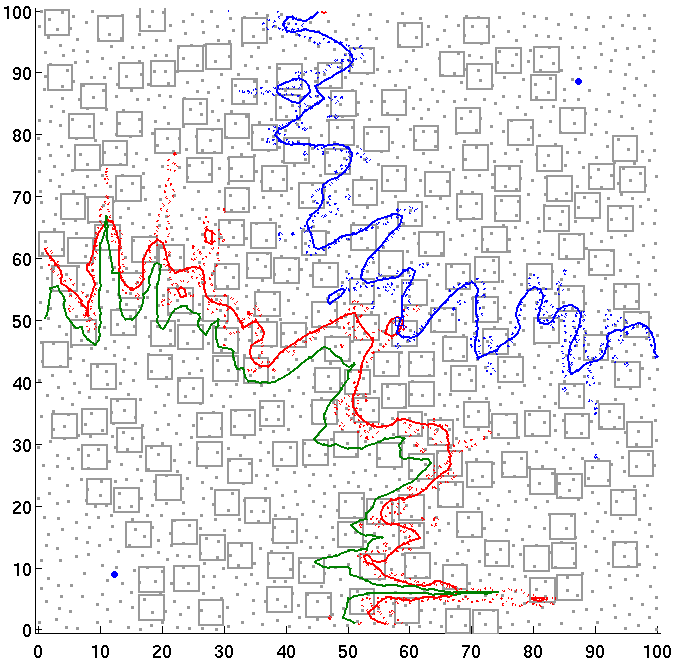
\includegraphics[scale=0.18]{figures/contribution1/vbNoOverlap}} 
\subfloat[]{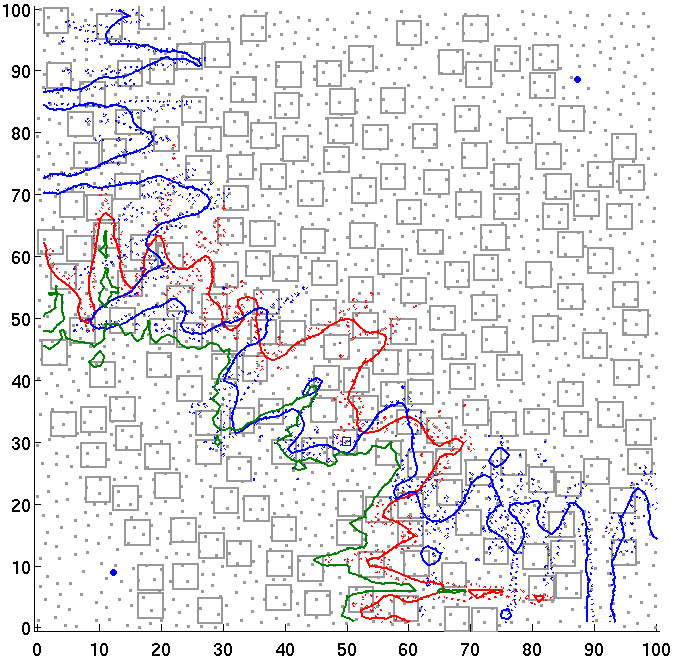
\includegraphics[scale=0.18]{figures/contribution1/vbOverlap}}
\caption{\label{fig:overlap} Demonstration of the effect of the overlap of the contours on the location probability. The results for this scenario are given in Tab.~\ref{tab:overlap} in terms of reduction of the location probability.}
\end{figure}

